%----------------------------------------------------------------------------------------
%	PACKAGES AND OTHER DOCUMENT CONFIGURATIONS
%----------------------------------------------------------------------------------------

\documentclass[twoside,twocolumn]{article}

\usepackage{blindtext} % Package to generate dummy text throughout this template 

\usepackage[numbers]{natbib}
\usepackage{dblfloatfix}
\usepackage[sc]{mathpazo} % Use the Palatino font
\usepackage[T1]{fontenc} % Use 8-bit encoding that has 256 glyphs
\linespread{1.05} % Line spacing - Palatino needs more space between lines
\usepackage{microtype} % Slightly tweak font spacing for aesthetics

\usepackage[utf8]{inputenc}	
\usepackage[english]{babel} % Language hyphenation and typographical rules

\usepackage{graphicx}
\usepackage{wrapfig}
\usepackage{float}
%\usepackage{subfigure}

\usepackage[hmarginratio=1:1,top=32mm,columnsep=20pt]{geometry} % Document margins
\usepackage[hang, small,labelfont=bf,up,textfont=it,up]{caption} % Custom captions under/above floats in tables or figures
\usepackage{subcaption}
\usepackage{booktabs} % Horizontal rules in tables

\usepackage{lettrine} % The lettrine is the first enlarged letter at the beginning of the text

\usepackage{enumitem} % Customized lists
\setlist[itemize]{noitemsep} % Make itemize lists more compact



\usepackage{abstract} % Allows abstract customization
\renewcommand{\abstractnamefont}{\normalfont\bfseries} % Set the "Abstract" text to bold
\renewcommand{\abstracttextfont}{\normalfont\small\itshape} % Set the abstract itself to small italic text

\usepackage{titlesec} % Allows customization of titles
\renewcommand\thesection{\Roman{section}} % Roman numerals for the sections
\renewcommand\thesubsection{\roman{subsection}} % roman numerals for subsections
\titleformat{\section}[block]{\large\scshape\centering}{\thesection.}{1em}{} % Change the look of the section titles
\titleformat{\subsection}[block]{\large}{\thesubsection.}{1em}{} % Change the look of the section titles

\usepackage{fancyhdr} % Headers and footers
\pagestyle{fancy} % All pages have headers and footers
\fancyhead{} % Blank out the default header
\fancyfoot{} % Blank out the default footer
\fancyhead[C]{Can mindfulness alter pain
sensitivity? $\bullet$ May 2018} % Custom header text
\fancyfoot[RO,LE]{\thepage} % Custom footer text

\usepackage{titling} % Customizing the title section

\usepackage[hidelinks]{hyperref} % For hyperlinks in the PDF

\renewcommand{\thetable}{\Roman{table}}
\renewcommand{\thefigure}{\Roman{figure}}


%----------------------------------------------------------------------------------------
%	TITLE SECTION
%----------------------------------------------------------------------------------------

\setlength{\droptitle}{-4\baselineskip} % Move the title up

\pretitle{\begin{center}\huge\bfseries} % Article title formatting
\posttitle{\end{center}} % Article title closing formatting
\title{Can mindfulness alter pain
sensitivity?} % Article title
\author{%
\textsc{Annabel Bantle, Irene Uriarte Mercader, Maria Kaalund Kroustrup}\\ % Your name
\textsc{and Toby Steven Waterstone}\\[1ex]
\normalsize Aalborg University \\ % Your institution
}

\date{May 31, 2018} % Leave empty to omit a date
\renewcommand{\maketitlehookd}{%
\begin{abstract}
IMPROVEMENTS !!!
\noindent \textbf{Objective:}
Studies show that mindfulness meditation provide the ability to enhance a broad spectrum of cognitive health outcomes on long-term mindfulness meditation on chronic pain patients. Nevertheless, there are not many studies which show the effect of short-term mindfulness for chronic neck pain. \textbf{Methods:} 
Pressure pain was applied with an algometer two times on healthy subjects, a control and treatment group, with a 5 days in between. The treatment group practiced 20 minutes of mindfulness meditation on 5 consecutive days between the two measurements, while the control group continued their normal routine.
\textbf{Results:} 
\textbf{Discussion:} 

\end{abstract}
}

%----------------------------------------------------------------------------------------

\begin{document}

% Print the title
\maketitle

%----------------------------------------------------------------------------------------
%	ARTICLE CONTENTS
%----------------------------------------------------------------------------------------

\section{Introduction}
Approximately 20~\% of the world population suffer from chronic pain \cite{Macfarlanea2016}. The characteristic of chronic pain is a duration of pain more than three months \cite{Mello2016}. Due to the persistence of pain the patients get restricted physically as well as psychically. The patients’ ability to participate in diverse activities decreases. Those activities are not only physical but also social, maintaining an independent lifestyle and relationships to friends and family can be affected. A survey in nine European countries by Breivik et al. \cite{Breivik2006} showed that pain has an impact on the work life, whereby 25\% of the patients indicated that they changed their job, responsibilities at job or lost their job due to chronic pain. Furthermore, depression was diagnosed in 21~\% of those patients. \cite{Breivik2006} 

One of the most common types of chronic pain is neck pain, as 25~\% suffer from this in the UK \cite{Macfarlanea2016}. Those patients are restricted by negatively affected fatigue and concentration \cite{vanRanderaat2016}. Furthermore, they suffer like the majority of chronic pain patients from anxiety and depressed mood, cognitive distress and the resulting physical limitations. \cite{Gross2013} 

At the moment there is no cure for chronic pain. The current treatment methods only provide possibilities to relieve the pain. \cite{Pope2017,marcus2009} Nevertheless, the majority of the patients feels pain daily and this pain increases throughout the day due to daily activities. \cite{Breivik2006} 
Chronic pain is mainly treated by medication. However, medications have side effects like abuse or organ damage. To avoid those risks, alternative methods can be used. \cite{Pope2017,marcus2009, stein2007} One of those methods is mindfulness meditation, which uses meditation as mental training to achieve diminished judgment of emotions, cognitive control and existential insight. \cite{marcus2009} There are several types of meditation techniques. One of the most common is  focused attention (FA), which is suitable for beginners and trains the concentration by focusing on an object or specific thing, often the sensation of breath. \cite{Zeidan2016, Kabat1982}. 

Previous studies show that mindfulness meditation was able to enhance a broad spectrum of cognitive health outcomes, such as improvements of emotion regulation, cognitive control and positive mode. Furthermore stress, depression and anxiety can be relieved. These improvements are due to practicing mindfulness meditation, especially because of the mental training in emotion regulation, cognitive control, acceptance and positive mood. \cite{marcus2009,Zeidan2012, Zeidan2016} Nevertheless, there are not many studies which investigating the effect of mindfulness meditation on chronic neck pain. \cite{Macfarlanea2016} Additionally, most studies investigated the outcomes of practicing mindfulness meditation over a time period of two months or longer. The effect of a shorter time period of mindfulness meditation on chronic neck pain is not investigated yet. 


The present study address if mindfulness FA meditation can alter pain sensitivity in the neck by measuring pressure pain threshold (Threshold) and pressure pain tolerance (Tolerance) in healthy subjects. Even though the study was conducted in healthy subjects, the sensation of the pain and the effects of meditation to the pain sensitivity can be transferred to chronic pain patients \cite{Kjogx2016}. The upper trapezius is involved in chronic neck pain and this muscle present lower pressure pain threshold values compared with other muscles \cite{Fischer1987, Falla2004}, wherefore it was chosen as location for pressure application.
Therefore the hypothesis \textit{"Short-term mindfulness FA meditation increases the Threshold and Tolerance in the right upper trapezius"} was tested.

%*** Write something about why we chose the upper trapezius - look into the problem formulation in WS ***


%------------------------------------------------

\section{Methods}
\subsection{Subjects}
42 healthy subjects, 21 female and 21 male were recruited (age: 23.93 $\pm$ 2.74 years, BMI: 23.66 $\pm$ 3.28). Subjects with ongoing meditation practice, acute or chronic pain, neurological, musculoskeletal or mental illness, pregnancy or taking medications that might influence their pain sensitivity were excluded.

\subsection{Study design}
A controlled trial was designed, whereby the subjects were assigned into a control and treatment group with an equal gender distribution, as illustrated in \autoref{fig:studydesign}.

\begin{figure}[H]
\centering
%\caption{} \vspace{-.25cm}
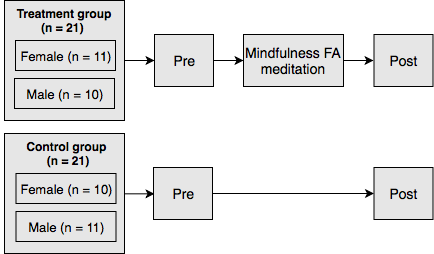
\includegraphics[width=1\columnwidth]{../figures/studydesign_aa.png}
\caption{Parallel study design, whereby subjects were assigned to either treatment or control group, striving an equal gender distribution. The treatment group was meditating on 5 consecutive days between the first (Pre) and second measurement (Post), whilst the control group continued their normal routine.}
\label{fig:studydesign}
\end{figure} 

\noindent 
The subjects of the treatment group practiced 20 minutes mindfulness FA meditation on 5 consecutive days between the two measurements, while the subjects of the control group continued their normal routine. The same time interval between the measurement sessions was used for the two groups.

\subsection{Measurements}%Experimental Procedure
The location where the pressure was applied shown in \autoref{fig:trapezius}, was marked at the right upper trapezius in the midpoint between the acromion and 7th cervical vertebra to ensure reliable and rapid location during the experimental procedure. 

Threshold and Tolerance were measured with an algometer (Wagner Force Ten™ Digital force Gage). Three repetitions with a 5 minutes resting period in between were conducted. The examiner was blinded during the measurements to avoid bias. The mean of the three repetitions, was computed as measurement value. 

\begin{figure}[H]
\centering
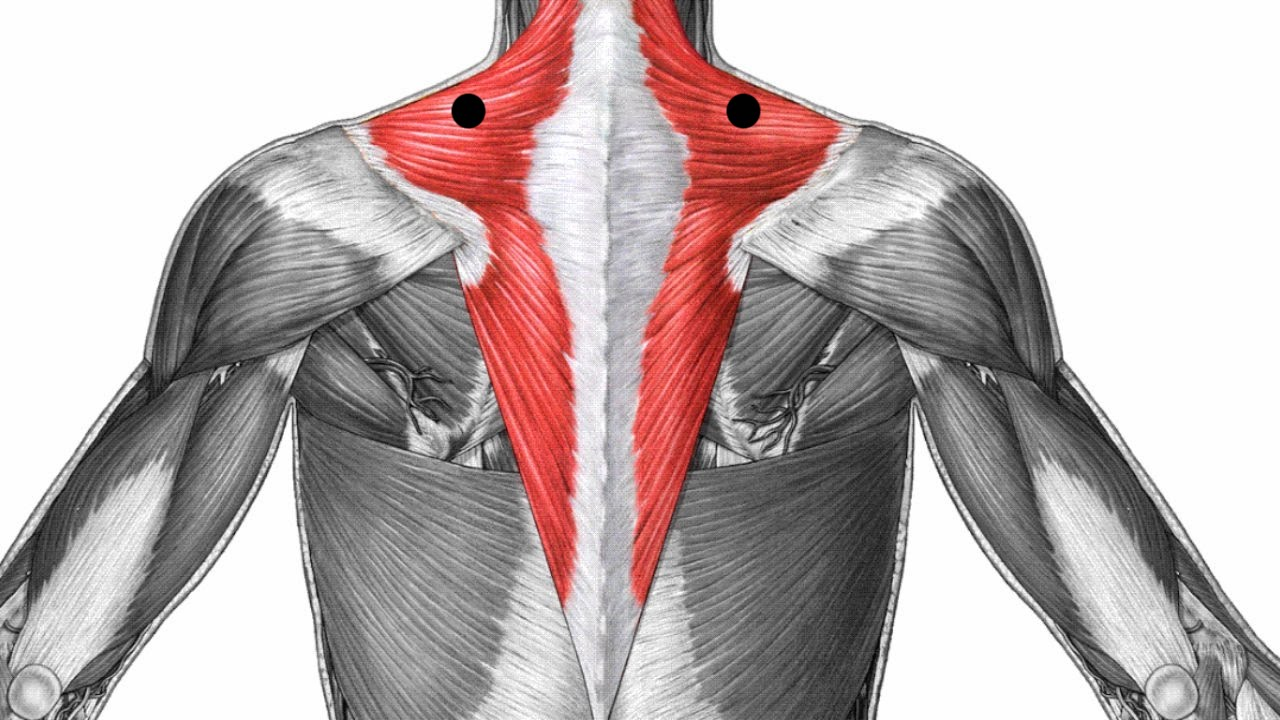
\includegraphics[width=.7\columnwidth]{../figures/trapezius}
\caption{Location of pressure application on the right upper trapezius marked with a black dot.}
\label{fig:trapezius}
\end{figure} \vspace{-.5cm}

%The treatment group practiced 20 minutes mindfulness meditation on 5 consecutive days. After the last meditation session the second measurement was conducted likewise the baseline measurement.
%The subjects of the control group continued their normal routine. The same time interval between baseline and second measurement was used for the subjects of the control group.

\subsection{Meditation Technique}
The treatment group practice short-term mindfulness FA meditation with 20 minutes of meditation on 5 consecutive days. To ensure same meditation conditions, a guided meditation in form of an audio file was used. The used meditation technique was FA focusing on the flow of breath. A short oral introduction to mindfulness FA meditation was provided before the first meditation session. 

\subsection{Data Analysis}
%At first the normality of the data sample was evaluated with a Shapiro-Wilk test. According to the outcome of the Shapiro-Wilk test, for comparison of treatment and control group with regards to threshold and tolerance of first and second measurement a two-way mixed ANOVA was applied. For comparison of the groups with regards to the difference in threshold and tolerance as a percentage of first and second measurement a t-test was applied.

At first the normality of the data samples was evaluated with a Shapiro-Wilk test and the equality of variances was evaluated with a Levene's test. 

According to the outcome of the Shapiro-Wilk test and the Levene’s test, ANOVA and t-test were chosen. The two-way mixed ANOVA was used, whereby factor 1 denotes the group of subjects, either treatment or control, and factor 2 denotes the measurement session, either the first (Pre) or the second (Post). Therewith the statistical significance of two variations was evaluated, the between-subjects variation in factor 1 and the within-subjects variation in factor 2. \cite{Mooi2018} Threshold and Tolerance have been analyzed with separate two-way mixed ANOVAs.

The t-test was used to compare the changes in Threshold and Tolerance between the measurement sessions of treatment and control group. Therefore the relative difference (Improvement) in Threshold and Tolerance between Pre and Post was calculated for each subject. A t-test was applied to the Improvements to test the mean difference between treatment and control group’s Improvement. \cite{Mooi2018} Threshold and Tolerance Improvements have been analyzed separately.




%------------------------------------------------

\section{Results}
The Tolerance for some of the subjects is not representative, as the examiner was not able to apply enough force with the algometer to reach the subjects' Tolerance, thus those subjects were excluded. 
Therefore the results are based on 32 subjects, 15 subjects in the treatment and 17 subjects in the control group. 

\subsection{Two-way Mixed ANOVA}
The Shapiro-Wilk test showed a normal distribution and the Levene's test showed equal variances for the Threshold and Tolerance Pre and Post for both, treatment and control group. Therefore the two-way mixed ANOVA was applied. Hereby the Pre and Post measurements of Threshold and Tolerance were compared to assess the within-subjects effect. The treatment and control group were compared to assess the between-subjects effect. The results from the two-way mixed ANOVA are illustrated in Table \ref{table:TWOWAYANOVA1} for Threshold and Table \ref{table:TWOWAYANOVA2} for the Tolerance. 

\begin{table}[ht]
\caption{Two-way mixed ANOVA for the Threshold Pre and Post for treatment and control group. P-values marked with an asterisk indicate significant difference. F-value and degree of freedom (df) are illustrated as well.}
\centering
\begin{tabular}{l c c c}
\toprule
\multicolumn{4}{c}{\textbf{Within-Subjects Effect}} \\
\midrule
& \textbf{df} &\textbf{F} & \textbf{p} \\ [0.5ex] % inserts table %heading
Measurement & 1 & 13.052 &  0.001* \\
Measurement x Group & 1 & 0.451 & 0.507 \\
\toprule
\multicolumn{4}{c}{\textbf{Between-Subjects Effect}} \\
\midrule 
& \textbf{df} & \textbf{F} & \textbf{p} \\ [0.5ex] % inserts table %heading
Group & 30 & 1.492 &  0.231 \\
\hline
\end{tabular}
\label{table:TWOWAYANOVA1}
\end{table}

The test indicates that there is a significant main effect between Pre and Post of the Threshold measurements (within-subject effect, Measurement), F(1,30) = 13.051, p = 0.001. However, no significant main effect is seen between the treatment and control group for Threshold (between-subjects effect, Group), F(1,30) = 1.492, p = 0.231 nor a significant main interaction between measurements and group (within-subjects effect, Measurement x Group), F(1,30) = 0.451, p = 0.507. 

\begin{table}[ht]
\caption{Two-way mixed ANOVA for the Tolerance Pre and Post for treatment and control group. P-values marked with an asterisk indicate significant difference. F-value and degree of
freedom (df) are illustrated as well.}
\centering
\begin{tabular}{l c c c}
\toprule
\multicolumn{4}{c}{\textbf{Within-Subjects Effect}} \\
\midrule  
& \textbf{df} & \textbf{F} & \textbf{p} \\ [0.5ex] % inserts table %heading
Measurement & 1 &  8.918 &  0.006* \\
Measurement x Group & 1 & 0.532 & 0.472 \\
\toprule
\multicolumn{4}{c}{\textbf{Between-Subjects Effect}} \\
\midrule
 & \textbf{df} & \textbf{F} & \textbf{p} \\ [0.5ex] % inserts table %heading
Group & 30 & 3.289 &  0.080 \\
\hline
\end{tabular}
\label{table:TWOWAYANOVA2}
\end{table}

\noindent
The test indicates that there is a significant main effect between Pre and Post of the Tolerance measurements (within-subject effect, Measurement), F(1,30) = 8.981, p=0.006. However, no significant main effect is seen between the treatment and control group for Threshold (between-subjects effect, Group), F(1,30) = 3.289, p = 0.080 nor a significant main interaction between  measurements and group (within-subjects effect, Measurement x Group), F(1,30) = 0.532, p = 0.472.

\subsection{T-test}
The Threshold and Tolerance increases for both, treatment and control group, between the measurements. The relative difference in Threshold and Tolerance is illustrated in Figure \ref{fig:barplot}. 

\begin{figure}[H]
\centering
%\caption{} \vspace{-.25cm}
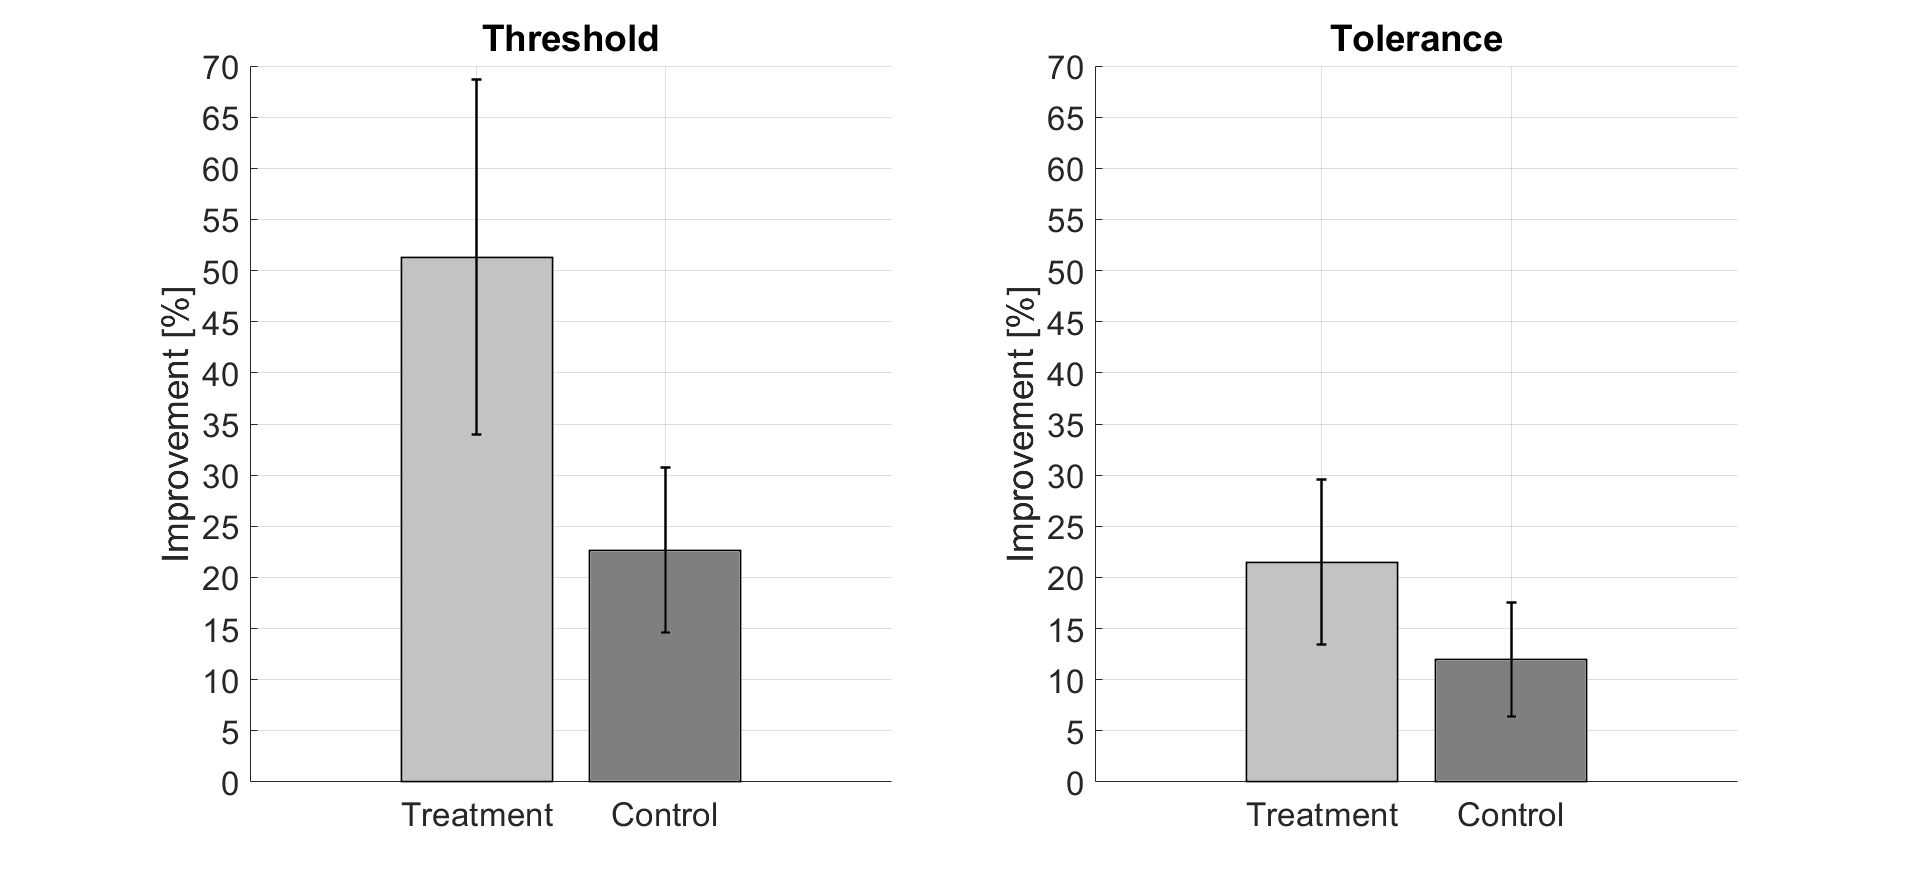
\includegraphics[width=1\columnwidth]{../figures/barplot.png}
\caption{Relative difference for Threshold (left) and Tolerance (right) with associated standard error for treatment group (light grey) and control group (dark grey).}
\label{fig:barplot}
\end{figure} 

The Shapiro-Wilk test showed a normal distribution. An unequal variance for the relative difference in Threshold and an equal variance for the relative difference in Tolerance was found for both groups. Therefore the t-test was applied. The results from the t-test are illustrated in Table \ref{table:TTEST}. 

\begin{table}[ht]
\caption{T-test for Threshold and Tolerance relative difference for treatment and control group. P-values marked with an asterisk indicate significant difference. F-value and degree of
freedom (df) are illustrated as well.}
\centering
\begin{tabular}{l c c} 
\toprule
\multicolumn{3}{c}{\textbf{Threshold}} \\
\midrule  
\textbf{df} & \textbf{F} & \textbf{p} \\ [0.5ex] % inserts table %heading
19.892 & 6.967 & 0.149    \\
\toprule
\multicolumn{3}{c}{\textbf{Tolerance}} \\
\midrule 
\textbf{df} & \textbf{F} & \textbf{p} \\ [0.5ex] % inserts table %heading
30 & 2.084 & 0.330 \\
\hline
\end{tabular}
\label{table:TTEST}
\end{table}

\noindent
The test indicates that there is no significant difference in the relative difference in Threshold, F(1,19.892) = 6.967, p = 0.149 and Tolerance, F(1,30) = 2.084, p = 0.330 between the groups.


%------------------------------------------------

\section{Discussion}

\subsection{Summary and Interpretation of the Findings}
%There was seen an overall increase in the threshold and tolerance within the two measurements for both, the treatment and control group. However, no significant improvement of the pressure pain threshold and pressure pain tolerance between the groups was found. Furthermore, no significant difference between the difference as a percentage in threshold and tolerance was found. But a tendency can be seen that the treatment group has a higher percentage increase in both threshold and tolerance compared with the control group. 

%A significant difference is found between the measurements, Pre and Post, indicated by the two-way mixed ANOVA. However, no significant difference in Threshold and Tolerance between treatment and control group is found. Furthermore, no significant difference in the relative difference in Threshold and Tolerance is found between the groups, indicated by the t-test. Nevertheless a tendency can be seen that the treatment group has a higher relative difference in Threshold and Tolerance compared with the control group. Hence the results show the habituation effect on pressure pain. A study by Bingel et al. \cite{Bingel2007} showed, that healthy subjects habituate to pain over time.  Furthermore a survey by Neddermeyer et al. \cite{Neddermeyer2007} found out that the pain threshold of a person does not depend on the stimulus source. 

A significant difference is found between Pre and Post measurement in treatment and control group, indicated by the two-way mixed ANOVA. This might be do to habituation to pressure pain. A study by Bingel et al. \cite{Bingel2007} showed, that healthy subjects habituate to heat pain over time.  Furthermore a survey by Neddermeyer et al. \cite{Neddermeyer2007} found that pain threshold does not depend on the source of the stimulus. Hence the results show the habituation effect to pressure pain.

However, no significant difference in Threshold and Tolerance between treatment and control group is found. Furthermore, no significant difference in relative difference in Threshold and Tolerance is found between the groups, indicated by the t-test. Nevertheless a tendency can be seen that the treatment group has a higher relative difference in Threshold and Tolerance compared with the control group. 

\subsection{Experimental Setup}
%More standardization of the experiment in some way… We rely on a person putting pressure on the subjects (Maybe own section: XXX)
%One of the drawbacks of the manual algometer is the difficulty in assessing objectively the rate in pressure applied. Different studies insist in the importance of training and practice with the algometer. However, due to the avaliable time to execute the project, an appropriate training period was not possible, which would be convenient in order to achieve reliable values.

The pressure application with an algometer should be conducted steady and consistent.
One of the drawbacks of the used algometer is the difficulty in accomplish this pressure
rate, since this algometer does not display a pressure rate.
%One of the drawbacks of the manual algometer is the difficulty in assessing objectively rate in pressure application. %, it is difficult to increase the pressure uniformly. 
%The examiner in charge of the experiment is a strong male, however he had difficulty to apply enough force to reach the pressure pain tolerance for some subjects. Some factors could affect this outcome like inappropriate technique using the algometer, examiner's fatigue after several measurements or the standing position during the experiment. 
According to Kinser et al. \cite{Kinser2009} and Vaughan et al. \cite{Vaughan2007} it is important to train and practice with the algometer.
However, due to the available time
to execute the project, an appropriate training period was not possible, which would be
convenient in order to achieve more representative values.
%However, due to the available time to execute the project, an appropriate training period was not possible, which would be convenient in order to achieve  more reliable values.
%Subjects: “ It’s hard to define the first sensation of pain.”
%Different subjects expressed difficulties ratting their own threshold, why it is challenging to find true values of pain. Hence, this research rely on the ability of the subjects to rate their pain.

%What if we only look at the threshold and not the tolerance. If you are a trained person you may have a higher tolerance compared to other subjects. 
%It appears more convenient to focus on the pressure pain threshold instead of the pressure pain tolerance, because of the big variability in tolerance measures and validity of the measures obtained from the subjects, because pain tolerance is harder to reach with the algometer.



%Pain tolerance is less used for research purposes due to ethical reasons as well as its high variability among the subjects \cite{Yarnitsky2006}. 

Pain tolerance values are highly altered by psychological and psychosocial factors, while pain threshold values seem to be relatively less
variable. Hence it appears convenient to only focus on the pain threshold. \cite{Yarnitsky2006}
%It appears convenient to only focus on the Threshold instead of the Tolerance. This is not only because of the extensive variety in the results, but also the validity of the measurements, as for some subjects it was not possible to reach a representative Tolerance.
%Would it have any influence if the subject should be sore in the muscle before the measurement due to training? (Yes, so an exclusion criteria would be not to train the muscle for maybe 2 days before the experiment)
%A study by Tesarz et al. \cite{Tesarz2012} concludes that pain perception can be altered by physical activity. Subjects with good physical condition participating in the study, showed higher threshold and tolerance values compared with other subjects. Nevertheless, this fact does not affect the outcomes of the study because we compared the subjects with themselves, not with the others.
%Along a study by Koltyn et al. \cite{Koltyn2002} concludes that high-intensity exercise is followed by hypoalgesia, which leads to an increased pain threshold as well as pain tolerance values during and after exercise. Based on this, the exclusion criteria should take into account that subjects cannot train before the measurement.

A study by Tesarz et al. \cite{Tesarz2012} concludes that pain perception can be altered by physical activity. This could be seen in our study as subjects with good physical condition showed higher Threshold and Tolerance values compared with other subjects.
 %The muscle of these subjects is also more appropriate to apply the pressure on.
%Nevertheless, this fact does not affect the outcomes of the study because we compared the subjects with themselves, not with the others. 
%Furthermore a study by Koltyn et al. \cite{Koltyn2002} determines that high-intensity exercise is followed by hypoalgesia. Therefore Threshold and Tolerance values increase during and after exercise. The exclusion criteria should take into account that subjects cannot practice physical exercise involving the upper part of the thorax before the measurements.
Furthermore a study by Koltyn et al. \cite{Koltyn2002} determines that high-intensity exercise is followed by hypoalgesia. Therefore Threshold and Tolerance values increase during and right after exercise \cite{Koltyn2002}. On the other hand Serinken et al. \cite{Serinken2013} showed that Threshold is decreased when applying pressure pain to sore muscles caused by physical exercise. Therefore the exclusion criteria should take into account that subjects cannot practice physical exercise right before or exorbitantly the days before a measurement session.

\subsection{Meditation Technique}
%Other studies have shown that mindfulness meditation has an effect on pain. Those studies investigated the effect of a meditation practice over two months or more using MBSR. \cite{Kabat1982,Rosenzweig2010} The effect on pain intensity and pain unpleasantness of short-term mindfulness meditation practice was shown by Zeidan et al. \cite{Zeidan2012}. However, Zeidan et al. \cite{Zeidan2012} used a meditation technique which was a combination of FA and OM, particularly focusing on pain-related brain processing. Whereas this study was investigating the effect of regular short-term mindfulness FA meditation. Hence one could speculate that different meditation types affect pain after various time periods of practice and that 5 consecutive days are not sufficient to elicit mindfulness FA meditation’s modulation of pain.

%Nevertheless, there were some limitations within the used meditation technique. Potentially the used audio-guide did not ensure that the subjects understood the principles of mindfulness FA meditation, even though an introduction to mindfulness meditation was given orally on the first day. However, this introduction was provided by a non-specialist, who possibly did not know the key focus of explaining mindfulness meditation to laymen. This uncertainty was based on board spectrum of mindfulness meditation techniques and their unclear delineations. 
%Furthermore, the subjects were told to meditate in the most comfortable position, which varied from subject to subject. These inconsistent sitting positions may have influenced the meditation outcome of single subjects. In addition, there was no control, if the subjects were meditating in the right way.
There were limitations within the used meditation technique. Potentially the used audio-guide did not ensure that the subjects understood the principles of mindfulness FA meditation, even though an oral introduction was given on the first day. However, this introduction was provided by a non-specialist, who possibly did not know the key focus of explaining mindfulness FA meditation to laymen. This uncertainty was based on the board spectrum of mindfulness meditation techniques and their unclear delineations. 

Furthermore, the subjects were told to meditate in the most comfortable position, which varied between the subjects. Inconsistent sitting positions may have influenced the meditation outcome of single subjects. In addition, there was no control, if the subjects were meditating adequately.

Other studies have shown that mindfulness meditation has an effect on pain. Those studies investigated the effect of meditation practice over two months or more using mindfulness-based stress reduction. \cite{Kabat1982,Rosenzweig2010} The effect on pain intensity and pain unpleasantness of short-term mindfulness meditation practice was shown by Zeidan et al. \cite{Zeidan2012}. However, Zeidan et al. \cite{Zeidan2012} used a meditation technique which combine FA and open monitoring, particularly focusing on pain-related brain processing. Whereas this study was investigating the effect of short-term mindfulness FA meditation. Hence pain relief is affected not only by the type of meditation but also by the practice period. Therefore 5 consecutive days may not be sufficient to elicit mindfulness FA meditation’s modulation of pain.

%------------------------------------------------

\section{Conclusion}
Short-term mindfulness FA meditation on 5 consecutive days did not show a significant effect on pressure pain relief in the upper trapezius. However, a significant effect was found between Pre and Post measurement for treatment and control group, which was seen as an increase in pressure pain.
Wherefore a clear conclusion on the effect of mindfulness FA meditation on pain relief cannot be stated. Nevertheless this study still contributes to the field of pain relief using mindfulness meditation as an alternative method. Since this study shows the tendency that 5 consecutive days of mindfulness FA meditation practices increase threshold and tolerance, a longer period should be investigated. Furthermore, this study indicates that the effects of mindfulness meditation varies depending on the meditation technique. Hence the effects of the different meditation techniques should be further investigated in order to evaluate if different meditation techniques provide various effects on pain relief. 

%----------------------------------------------------------------------------------------
%	REFERENCE LIST
%----------------------------------------------------------------------------------------


\footnotesize{\bibliographystyle{unsrt}
\bibliography{C:/Users/tobbe/Documents/GitHub/BMEI-2.sem/setup/BMEI_2.sem}


%\endgroup

%----------------------------------------------------------------------------------------

\end{document}
